\documentclass[a4paper]{article}

\usepackage[margin=1in]{geometry}    
\usepackage[english]{babel}
\usepackage[utf8]{inputenc}
\usepackage[noend]{algpseudocode}
\usepackage{hyperref}
\usepackage{fancyhdr}
\usepackage{algorithm}
\usepackage{arevmath}
\usepackage{mathtools}   
\usepackage{graphicx}
\graphicspath{ {./Figures/} }  
%opening
\title{Improving Interpretability in Symbolic Regression Models Using Multi-objective GP and the Transient Terminal Set}
\author{Asher Stout, 300432820}

\begin{document}
\maketitle

%Description of initial work & hours spent
\section{Overview of Work \& Research}
\paragraph{} Work began on the project with research into previous approaches for improving the interpretability of Symbolic Regression models, and ultimately Multi-objective GP (MOGP) was selected as an area for further study. Several relevant papers defined the interpretability of a solution as the depth or size of its tree representation, which may not accurately correlate to its computational complexity. Thus, it was decided that a new measure of complexity be developed for use in MOGP. In addition, the entirely random nature of mutation operators in MOGP was identified as a place for potential innovation in improving Symbolic Regression model interpretability. This resulted in a new approach being developed called the \textbf{Transient Terminal Set}, which is described in further detail in \textbf{Section 2}.
\paragraph{} Aside from research, extensive time was invested into learning the tools required for the completion of the project objectives - particularly Python, DEAP, and LaTeX. This involved practical applications in the form of tutorials and implementing a standard MOGP and culminated in the formal definition of the Transient Terminal Set algorithm (see \textbf{Section 2}) and its implementation using DEAP (see \textbf{Section 3}). 
\paragraph{}The total hours spent on the project, as of 11 January 2021, were \textbf{196}.

%Basically the algorithm contained in TTSGP_Algorithm, with some minor formatting adjustments
\section{Transient Terminal Set}
\begin{algorithm}
	\caption{Multi-objective GP using the Transient Terminal Set (TTSGP)}
	\hspace*{\algorithmicindent} \textbf{Input:} population size \(\rho\), crossover probability \textit{p$_{c}$}, mutation probability \textit{p$_{m}$}, transient mutation probability \textit{p$_{d}$}, terminal set \(T\), function set \(F\), death age \(\alpha\) \\
	\hspace*{\algorithmicindent} \textbf{Define:} generation \(G_{n}\), individual fitness \(f_{i}\), transient terminal set \(M_{G_{n}}\), fitness threshold \(f_{t, G_{n}}\) \\ 
	\begin{algorithmic}[1]
		\State Initialize starting population \textit{$ P_{G_{0}} $}, \(M_{G_{0}}\leftarrow \emptyset\), \(f_{t, G_{0}} \leftarrow 0\)
		\While{\textit{no improvement in} \(\max f_{i}\in P_{G_{n}}\) \textit{since} \(P_{G_{n-5}}\)} \Comment{Evolve generation  \(G_{n+1}\)}
		\State \(P_{G_{n+1}}\leftarrow \emptyset\), \(M_{G_{n+1}}\leftarrow M_{G_{n}}\)
		\While{len\(P_{G_{n+1}} \neq \rho\)}	\Comment{Update population \(P_{G_{n+1}}\)}
		\State Perform crossover $\forall i\in P_{G_{n}}$ with \textit{p$_{c}$}
		\State Perform mutation $\forall i\in P_{G_{n}}$ with \textit{p$_{m}$}, \(T\), \(F\)
		\State Perform transient mutation $\forall i\in P_{G_{n}}$ with \textit{p$_{d}$, \(M_{G_{n}}\)}
		\State $P_{G_{n+1}} \leftarrow P_{G_{n+1}}\cup \{i | i_{offspring}\}$
		\EndWhile\newline
		\ForAll{subtree \(s \in  M_{G_{n+1}}\)}	\Comment{Update transient terminal set \(M_{G_{n+1}}\)}
		\If{\(age(s) > \alpha\)}
		\State Prune \(s\) from \(M_{G_{n+1}}\)
		\EndIf
		\EndFor
		\State Compute $f_{t, G_{n}}$ from $\forall f_{i} \in P_{G_{n+1}}$
		\For{$i\in P_{G_{n+1}}$}	
		\State $f_{c}\leftarrow \Delta f_{i}$ from \(G_{n}\) to \(G_{n+1}\)
		\If{ $f_{c} > $ \(f_{t, G_{n}}\)}
		\State \(M_{G_{n+1}} \leftarrow M_{G_{n+1}} \cup \{\)subtree \(s\in i \}\)
		\EndIf
		\EndFor 
		\EndWhile
\end{algorithmic}\end{algorithm}
%Provide reasoning for why the algorithm will improve interpretability
\paragraph{Note:} The transient terminal set is utilized during a genetic operation called \textit{transient mutation}, in which a candidate solution is mutated with a member of the set. The transient terminal set is composed of subtrees generated in the population (either through crossover or normal mutation) which have resulted in substantial increases in the fitness of candidate solutions.
\paragraph{} The Transient Terminal Set seeks to improve the interpretability of Symbolic Regression models via the use of multi-objective GP by improving the search process itself. By utilizing a complexity measure in addition to an error measure as the Pareto-efficient objectives for the algorithm, and pairing this with the proposed transient terminal set, it is theorized that candidate solutions will become less complex when compared with standard multi-objective GP. As the selection process for the transient terminal set follows this multi-objective framework, improvements in either objective will result in a candidate solution's altered subtree being added to the set. Thus, the transient terminal set distributes proven subtrees that result in lower errors and/or complexities throughout the population. This process potentially results in candidate solutions with both minimized error and complexity measures, and is an improvement over the entirely randomized mutation of standard multi-objective GP.

%From initial experimentation; graphs were generated using matplotlib and networkx/pygraphviz
\section{Experimentation Results}
\paragraph{Note:} The code for this experiment can be accessed at \url{https://github.com/VeryEager/transient-terminal-gp}. The experiments utilized the following datasets: Red Wine Quality, White Wine Quality, Concrete Strength, Boston House Price, and Bike Rentals (preprocessed). No additional preprocessing was performed on the datasets prior to experimentation, with the exceptions of the removal of a constant feature in the Boston House Price data and the removal of the 'datetime' feature in the Bike data. Both these features were determined irrelevant.

%Comparison of Evolutions in all data sets
\begin{figure}[H]
	\caption{Evolution using Standard MOGP, winequality-red}
	\centering
	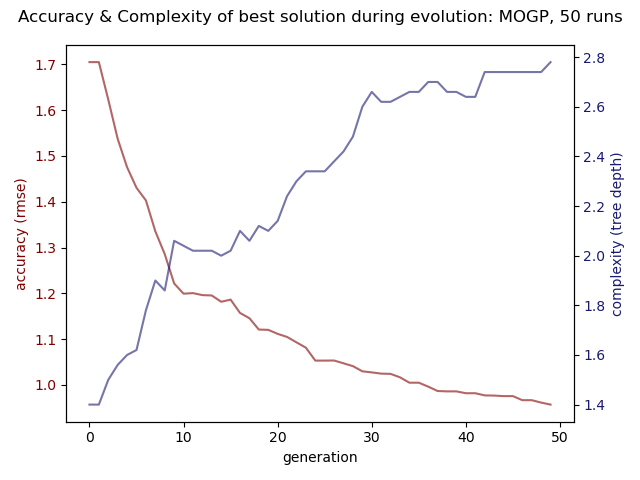
\includegraphics[width=0.875\textwidth]{winequality-red-evo-MOGP}
\end{figure}
\begin{figure}[H]
	\caption{Evolution using Transient Terminal Set GP, winequality-red}
	\centering
	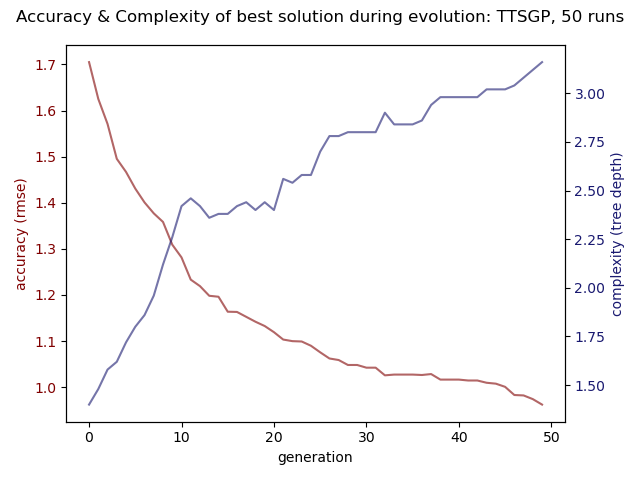
\includegraphics[width=0.875\textwidth]{winequality-red-evo-TTSGP}
\end{figure}
\begin{figure}[H]
	\caption{Evolution using Standard MOGP, winequality-white}
	\centering
	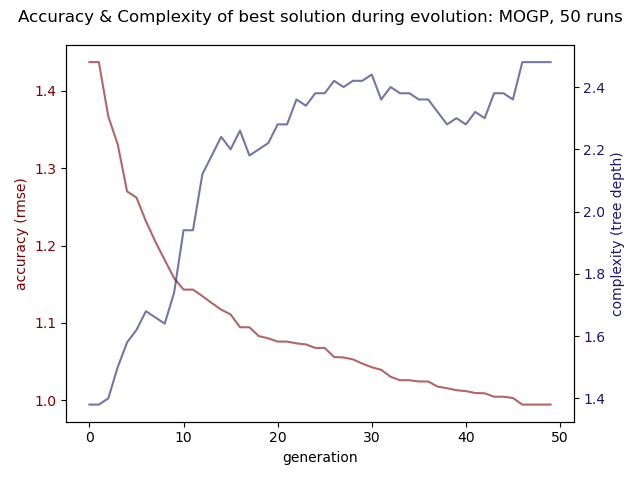
\includegraphics[width=0.875\textwidth]{winequality-white-evo-MOGP}
\end{figure}
\begin{figure}[H]
	\caption{Evolution using Transient Terminal Set GP, winequality-white}
	\centering
	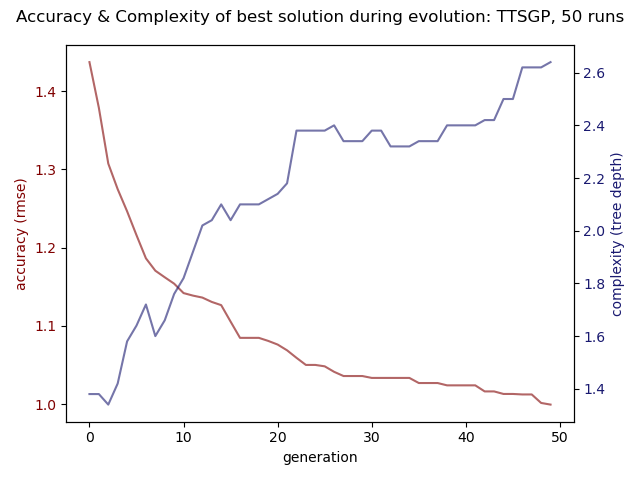
\includegraphics[width=0.875\textwidth]{winequality-white-evo-TTSGP}
\end{figure}
\begin{figure}[H]
	\caption{Evolution using Standard MOGP, strength-concrete}
	\centering
	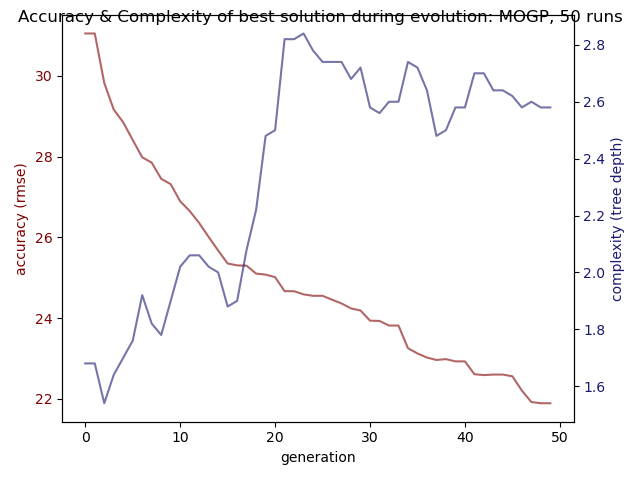
\includegraphics[width=0.875\textwidth]{strength-concrete-evo-MOGP}
\end{figure}
\begin{figure}[H]
	\caption{Evolution using Transient Terminal Set GP, strength-concrete}
	\centering
	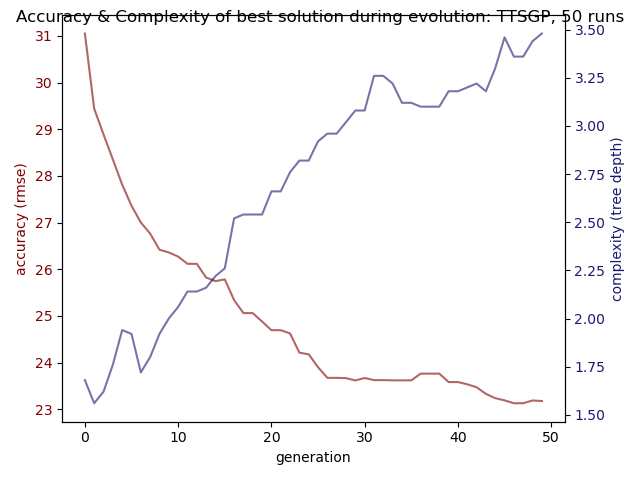
\includegraphics[width=0.875\textwidth]{strength-concrete-evo-TTSGP}
\end{figure}
\begin{figure}[H]
	\caption{Evolution using Standard MOGP, houseprice-boston}
	\centering
	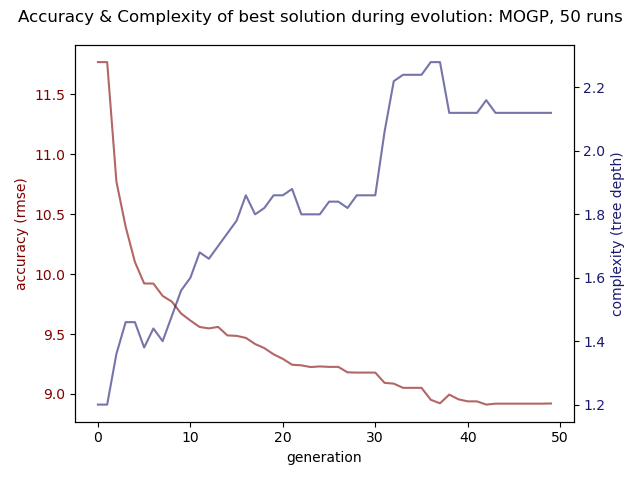
\includegraphics[width=0.875\textwidth]{houseprice-boston-evo-MOGP}
\end{figure}
\begin{figure}[H]
	\caption{Evolution using Transient Terminal Set GP, houseprice-boston}
	\centering
	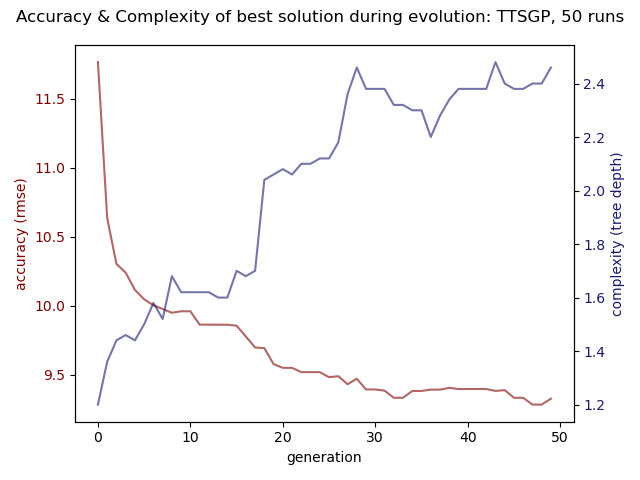
\includegraphics[width=0.875\textwidth]{houseprice-boston-evo-TTSGP}
\end{figure}
\begin{figure}[H]
	\caption{Evolution using Standard MOGP, estcount-bike}
	\centering
	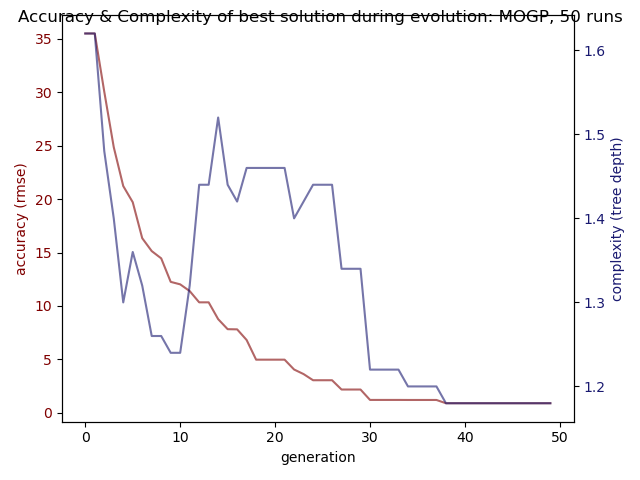
\includegraphics[width=0.875\textwidth]{estcount-bike-evo-MOGP}
\end{figure}
\begin{figure}[H]
	\caption{Evolution using Transient Terminal Set GP, estcount-bike}
	\centering
	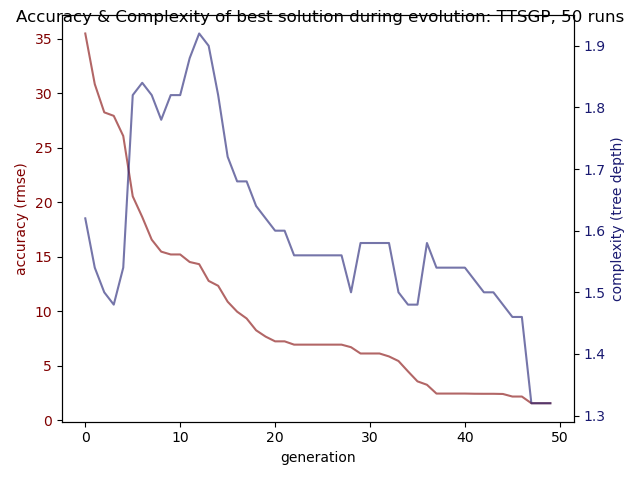
\includegraphics[width=0.875\textwidth]{estcount-bike-evo-TTSGP}
\end{figure}

%Comparison of solutions in red wine data
\begin{figure}[H]
	\caption{Best individual in Standard MOGP Evolution, winequality-red}
	\centering
	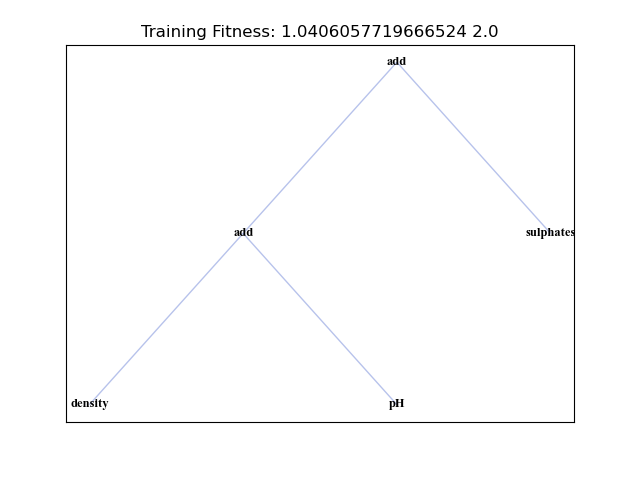
\includegraphics[width=0.875\textwidth]{winequality-red-MOGP-ex}
\end{figure}
\begin{figure}[H]
	\caption{Best individual in TTSGP Evolution, winequality-red}
	\centering
	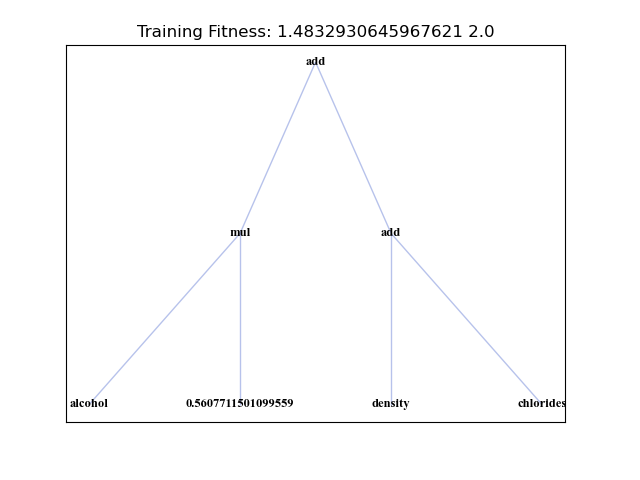
\includegraphics[width=0.875\textwidth]{winequality-red-TTSGP-ex}
\end{figure}
\paragraph{}The parameters for the experiment were \textit{generations} = 50, \textit{population} = 100, \textit{crossover probability} = 0.5, \textit{mutation probability} = 0.1, and \textit{transient mutation probability} = 0.1. The dataset was split into 70\% training instances and 30\% testing instances prior to evolution. Results for the techniques were averaged across 50 random seeds, and the resulting evolution of the averaged best individual are plotted in \textbf{Figures 1 through 10} for each dataset. \textbf{Figure 3} and \textbf{Figure 4} are the best individuals for one of the random seeds (661477758) in the Red Wine Quality dataset, and serve to illustrate the symbolic regression trees generated by both techniques. A full list of the seeds used during experimentation can be obtained from the file \textit{shared.py} in the aforementioned git repository. 
\paragraph{} The results in \textbf{Figures 1 through 10} suggest TTSGP is competitive with Standard MOGP but does not result in improvement in either the accuracy or complexity measures. Across all 5 datasets TTSGP achieved an RMSE approximately equal to the RMSE produced during Standard MOGP or slightly higher, however the tree depth of TTSGP solutions was consistently higher than Standard MOGP, generally within 0.25 nodes greater on average (except for in the case of the Concrete Strength data). This is in contrast to an earlier experiment performed on the Red Wine Quality dataset, which suggested a marginal improvement over Standard MOGP.
\paragraph{} There are several hypothetical factors which may have caused the poor performance of TTSGP. 
\begin{itemize}
	\item First, the chosen \textit{transient mutation probability} may be inadequate for symbolic regression. The current value of 10\% was arbitrarily chosen to match the \textit{mutation probability}, and further experimentation must be performed to determine whether any improvement can be made by adjusting \textit{tmutpb}. 
	\item Second, the rules for adding subtrees to the TTS may also be overly lenient, as the currently implemented mean approach is heavily susceptible to outliers. As with the mutation probability, further experimentation must be done to determine whether any improvement can be made through adjustment of this approach. 
	\item Finally, the TTSGP approach may be incomplete in its current state. Further extensions can be made to the algorithm to improve the results. Most notably, these are selecting the node to mutate within a tree via a heuristic function based on node depth (the current implementation utilizes an equal probability for each node) and selecting the member of the TTS to mutate in based on the tree topography at the selected node (the current implementation selects a random member of the TTS).
\end{itemize}

%From the ideas document
\section{Intended Future Work}
While the majority of the Transient Terminal Set algorithm is already implemented, there are several noteworthy aspects which need to be further investigated or developed to improve the results of TTSGP experimentation. \begin{itemize}
	\item As mentioned in \textbf{Section 3}, further experimentation will be done to analyze the effectiveness of raising or lowering the transient mutation probability on a generated solution's accuracy \& complexity.
	\item Second, the criteria for a subtree to be added to the set will be adjusted, as the currently-implemented mean approach is very susceptible to outliers. Experimentation will be performed to investigate which alternative (median, percentile, etc) is best suited for this problem.
	\item Third, as mentioned in \textbf{Section 1}, a more appropriate measure of model complexity will be created to ensure candidate solutions in TTSGP are actually less complex than those generated in standard MOGP.
	\item Fourth, further research and experimentation into the \textit{probability of node insertion} and \textit{probability of terminal selection during transient mutation} will be undertaken, as these concepts are closely linked with the Transient Terminal Set.
\end{itemize}
As of \textbf{1/4/20}, major bugfixes and general improvements to the project code have been made and rendered the initial results, presented on 12/15/2020, irrelevant.

\end{document}
